\documentclass{article}
\usepackage{lmodern}
\usepackage[T1]{fontenc}
\usepackage{shapepar}
\usepackage{microtype}
\usepackage{lipsum}
\usepackage{pgfplots}
\pgfplotsset{compat=1.9}
\usepackage{tikz}
\usetikzlibrary{calc,fit,intersections,folding}
\usepackage{pstricks-add}
\usetikzlibrary{arrows.meta,angles,arrows,quotes,backgrounds}
\usepackage[top = 5mm, bottom = 5mm]{geometry}

\newcommand{\tubecolor}{blue}
\newcommand{\thickness}{0.5mm}
\newcommand{\n}{2mm}

\begin{document}
\thispagestyle{empty}
\begin{center}
    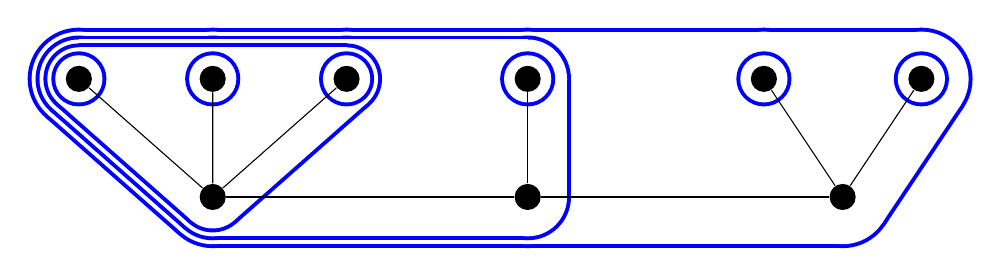
\begin{tikzpicture}

    
\begin{scope}
        \node[fill, circle] (1) at (0,0) [circle] {};
        \node[fill, circle] (2) at (4,0) [circle] {};
        \node[fill, circle] (3) at (8,0) [circle] {};

        \node[fill, circle] (11) at (-1.7,1.5) {};
        \node[fill, circle] (12) at (0,1.5) {};
        \node[fill, circle] (13) at (1.7,1.5) {};

        \node[fill, circle] (21) at (4,1.5) {};

        \node[fill, circle] (31) at (7,1.5) {};
        \node[fill, circle] (32) at (9,1.5) {};

        \draw (1) -- (2) -- (3);
        \draw (1) -- (11) (1) -- (12) (1) -- (13);
        \draw (2) -- (21);
        \draw (3) -- (31) (3) -- (32);
%1 11 12 13 2 21 3 31 32
        \begin{scope}[on background layer]
            \fill[\tubecolor] (1) circle (\n + 9*\thickness);
            \fill[\tubecolor] (11) circle (\n + 9*\thickness);
            \fill[\tubecolor] (12) circle (\n + 9*\thickness);
            \fill[\tubecolor] (13) circle (\n + 9*\thickness);
            \fill[\tubecolor] (2) circle (\n + 9*\thickness);
            \fill[\tubecolor] (21) circle (\n + 9*\thickness);
            \fill[\tubecolor] (3) circle (\n + 9*\thickness);
            \fill[\tubecolor] (31) circle (\n + 9*\thickness);
            \fill[\tubecolor] (32) circle (\n + 9*\thickness);
            \draw[\tubecolor] [line width = 2*(\n + 9*\thickness)] (1.center) -- (11.center);
            \draw[\tubecolor] [line width = 2*(\n + 9*\thickness)] (11.center) -- (32.center);
            \draw[\tubecolor] [line width = 2*(\n + 9*\thickness)] (32.center) -- (3.center);
            \draw[\tubecolor] [line width = 2*(\n + 9*\thickness)] (3.center) -- (1.center);
            
            \fill[white] (1) circle (\n + 8*\thickness);
            \fill[white] (11) circle (\n + 8*\thickness);
            \fill[white] (12) circle (\n + 8*\thickness);
            \fill[white] (13) circle (\n + 8*\thickness);
            \fill[white] (2) circle (\n + 8*\thickness);
            \fill[white] (21) circle (\n + 8*\thickness);
            \fill[white] (3) circle (\n + 8*\thickness);
            \fill[white] (31) circle (\n + 8*\thickness);
            \fill[white] (32) circle (\n + 8*\thickness);
            \draw[white] [line width = 2*(\n + 8*\thickness)] (1.center) -- (11.center);
            \draw[white] [line width = 2*(\n + 8*\thickness)] (11.center) -- (32.center);
            \draw[white] [line width = 2*(\n + 8*\thickness)] (32.center) -- (3.center);
            \draw[white] [line width = 2*(\n + 8*\thickness)] (3.center) -- (1.center);
            \fill[white] (1.center) -- (11.center) -- (32.center) -- (3.center) -- (1.center);
        \end{scope}
%1 11 12 13 2 21
        \begin{scope}[on background layer]
            \fill[\tubecolor] (1) circle (\n + 7*\thickness);
            \fill[\tubecolor] (11) circle (\n + 7*\thickness);
            \fill[\tubecolor] (12) circle (\n + 7*\thickness);
            \fill[\tubecolor] (13) circle (\n + 7*\thickness);
            \fill[\tubecolor] (2) circle (\n + 7*\thickness);
            \fill[\tubecolor] (21) circle (\n + 7*\thickness);
            \draw[\tubecolor] [line width = 2*(\n + 7*\thickness)] (1.center) -- (11.center);
            \draw[\tubecolor] [line width = 2*(\n + 7*\thickness)] (11.center) -- (13.center);
            \draw[\tubecolor] [line width = 2*(\n + 7*\thickness)] (13.center) -- (21.center);
            \draw[\tubecolor] [line width = 2*(\n + 7*\thickness)] (21.center) -- (2.center);
            \draw[\tubecolor] [line width = 2*(\n + 7*\thickness)] (2.center) -- (1.center);
            
            \fill[white] (1) circle (\n + 6*\thickness);
            \fill[white] (11) circle (\n + 6*\thickness);
            \fill[white] (12) circle (\n + 6*\thickness);
            \fill[white] (13) circle (\n + 6*\thickness);
            \fill[white] (2) circle (\n + 6*\thickness);
            \fill[white] (21) circle (\n + 6*\thickness);
            \draw[white] [line width = 2*(\n + 6*\thickness)] (1.center) -- (11.center);
            \draw[white] [line width = 2*(\n + 6*\thickness)] (11.center) -- (13.center);
            \draw[white] [line width = 2*(\n + 6*\thickness)] (13.center) -- (21.center);
            \draw[white] [line width = 2*(\n + 6*\thickness)] (21.center) -- (2.center);
            \draw[white] [line width = 2*(\n + 6*\thickness)] (2.center) -- (1.center);
            \fill[white] (1.center) -- (11.center) -- (13.center) -- (21.center) -- (2.center) -- (1.center);
        \end{scope}
%1 11 12 13
        \begin{scope}[on background layer]
            \fill[\tubecolor] (1) circle (\n + 5*\thickness);
            \fill[\tubecolor] (11) circle (\n + 5*\thickness);
            \fill[\tubecolor] (12) circle (\n + 5*\thickness);
            \fill[\tubecolor] (13) circle (\n + 5*\thickness);
            \draw[\tubecolor] [line width = 2*(\n + 5*\thickness)] (1.center) -- (11.center);
            \draw[\tubecolor] [line width = 2*(\n + 5*\thickness)] (11.center) -- (13.center);
            \draw[\tubecolor] [line width = 2*(\n + 5*\thickness)] (13.center) -- (1.center);
            
            \fill[white] (1) circle (\n + 4*\thickness);
            \fill[white] (11) circle (\n + 4*\thickness);
            \fill[white] (12) circle (\n + 4*\thickness);
            \fill[white] (13) circle (\n + 4*\thickness);
            \draw[white] [line width = 2*(\n + 4*\thickness)] (1.center) -- (11.center);
            \draw[white] [line width = 2*(\n + 4*\thickness)] (11.center) -- (13.center);
            \draw[white] [line width = 2*(\n + 4*\thickness)] (13.center) -- (1.center);
            \fill[white] (1.center) -- (11.center) -- (13.center) -- (1.center);
        \end{scope}

%singletons
        \begin{scope}[on background layer]
            \foreach \x in {11,12,13,21,31,32} {
                \fill[\tubecolor] (\x) circle (\n + 3*\thickness);
                \fill[white] (\x) circle (\n + 2*\thickness);
            }
        \end{scope}
    \end{scope}    
    \end{tikzpicture}
    \end{center}
\end{document}

%1 11 12
        \begin{scope}[on background layer]
            \fill[\tubecolor] (1) circle (\n + 7*\thickness);
            \fill[\tubecolor] (11) circle (\n + 7*\thickness);
            \fill[\tubecolor] (12) circle (\n + 7*\thickness);
            \draw[\tubecolor] [line width = 2*(\n + 7*\thickness)] (1.center) -- (11.center);
            \draw[\tubecolor] [line width = 2*(\n + 7*\thickness)] (1.center) -- (12.center);
            \draw[\tubecolor] [line width = 2*(\n + 7*\thickness)] (11.center) -- (12.center);
            
            \fill[white] (1) circle (\n + 6*\thickness);
            \fill[white] (11) circle (\n + 6*\thickness);
            \fill[white] (12) circle (\n + 6*\thickness);
            \draw[white] [line width = 2*(\n + 6*\thickness)] (1.center) -- (11.center);
            \draw[white] [line width = 2*(\n + 6*\thickness)] (1.center) -- (12.center);
            \draw[white] [line width = 2*(\n + 6*\thickness)] (11.center) -- (12.center);
            \fill[white] (1.center) -- (11.center) -- (12.center) -- (1.center);
        \end{scope}
%1 11
        \begin{scope}[on background layer]
            \fill[\tubecolor] (1) circle (\n + 5*\thickness);
            \fill[\tubecolor] (11) circle (\n + 5*\thickness);
            \draw[\tubecolor] [line width = 2*(\n + 5*\thickness)] (1.center) -- (11.center);
            
            \fill[white] (1) circle (\n + 4*\thickness);
            \fill[white] (11) circle (\n + 4*\thickness);
            \draw[white] [line width = 2*(\n + 4*\thickness)] (1.center) -- (11.center);
        \end{scope}